%----------------------------------------------------------
\chapter{Постановка задачи}
%----------------------------------------------------------
\section{Требования к графовому модулю comsdk}\label{section:requirements}
Концептуальная постановка задачи.

Для описания процесса решения задачи в виде графа в программном каркасе GBSE был разработан специальный текстовый формат \gls{aDOT}. Он построен на основе распространённого языка описания графов Dot (Graphviz)\cite{GraphvizDot2022}. Основным его отличием является необходимость хранить помимо узлов, рёбер и их атрибутов дополнительную информацию о вызываемых в процессе обхода графовой модели функций, а именно:
\begin{itemize}
    \item тип функции -- обработчик, предикат, селектор;
    \item путь к библиотеке, из которой можно извлечь данную функцию;
    \item идентификатор.
\end{itemize}
Подробное описание этого формата приведено в~\cite{SokolovADOT2020}.
Ниже приведён пример описания графовой модели на языке aDot (листинг \ref{lst:aDotExample})
\begin{lstlisting}[label={lst:aDotExample}, caption={Пример описания графовой модели на языке aDot}]
digraph SIMPLEST {
    FUNCA [module=libtest, entry_func=IncA]
    FUNCB [module=libtest, entry_func=IncB]
    
    CHECKA [module=libtest, entry_func=CheckAEq4]
    CHECKB [module=libtest, entry_func=CheckBEq4]
    
    SETA [module=libtest, entry_func=SetAEq1]
    SETB [module=libtest, entry_func=SetBEq1]

    PASS [module=libtest, entry_func=PassFunc]
    PRED [module=libtest, entry_func=PassPred]

    INCR_A [predicate=PRED, function=FUNCA]
    INCR_B [predicate=PRED, function=FUNCB]
    CH_A [predicate=CHECKA, function = PASS]
    SET_A [predicate=PRED, function=SETA]
    SET_B [predicate=PRED, function=SETB]
    CH_B [predicate=CHECKB, function = PASS]
    
    __BEGIN__ -> ROT [morphism=SET_A]
    ROT -> ROOT[morphism=SET_B]
    ROOT ->  BR1, BR2 [morphism=(INCR_A, INCR_B)]
    BR1 -> BR1_ST [morphism=INCR_A]
    BR2 -> BR2_ST [morphism=INCR_B]
    BR1_ST, BR2_ST -> MERGE [morphism=(INCR_A, INCR_B)]
    MERGE -> __END__, __END__ [morphism=(CH_A, CH_B)]
}
\end{lstlisting}

В данном описании объявляются функции-обработчики \textsf{PASS}, \textsf{FUNCA}, \textsf{FUNCB}, \textsf{SETA} и \textsf{SETB} и функции-предикаты \textsf{CHECKA}, \textsf{CHECKB} и \textsf{PRED}, которые можно найти в библиотеке \textsf{libtest}. Кроме того, объявляются морфизмы, содержащие предикаты и обработчики. На рисунке~\ref{fig:aDotExample} изображено визуальное представление модели, описанной выше с некоторыми пояснениями.
\begin{figure}[!ht]
    \centering
    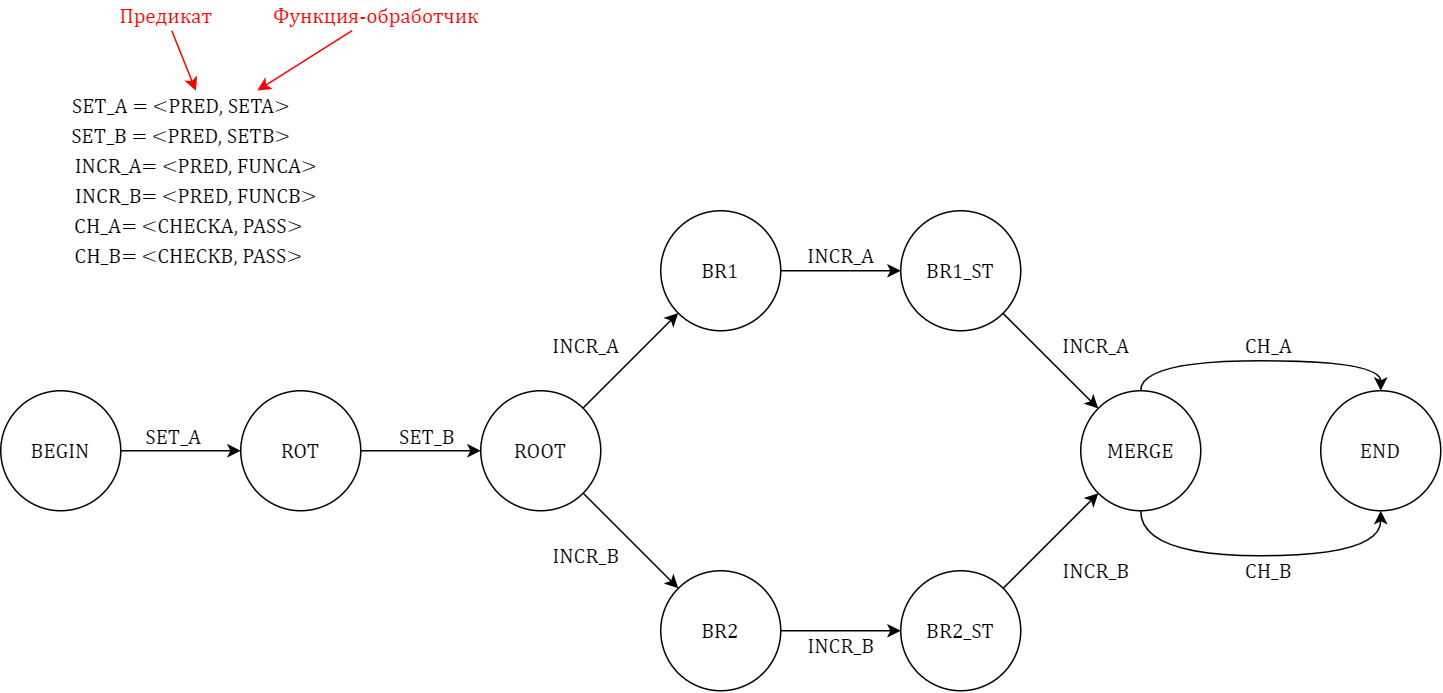
\includegraphics[width=\textwidth]{figures/adot_example.png}
    \caption{Пример графовой модели}
    \label{fig:aDotExample}
\end{figure}

В результате анализа текущего синтаксиса языка aDOT были сформулированы следующие требования к структуре графовых моделей в новой версии графового модуля библиотеки comsdk:
\begin{enumerate}[1)]
    \item Каждое ребро графа должно иметь возможность привязать к нему до трёх морфизмов -- препроцессор, обработчик и постпроцессор;
    \item Каждый морфизм должен содержать в себе функцию-предикат и функцию-обработчик;
    \item Каждый узел графа должен хранить состояние данных (т.е. сведения о типах и именах переменных);
    \item Каждый узел графа должен иметь возможность привязать к нему функцию-селектор;
    \item Каждый узел графа должен хранить данные о стратегии выполнения рёбер, исходящих из него (поочерёдное выполнение, выполнение в отдельных потоках, выполнение в отдельных процессах, выполнение на удалённом узле через SSH-подключение);
\end{enumerate}

%----------------------------------------------------------
\section{Анализ текущей версии графового модуля comsdk}
%----------------------------------------------------------
На рисунке~\ref{fig:oldGraphStructure} представлена UML-диаграмма классов, связанных с представлением в comsdk ориентированного графа, описывающего организацию вычислительных процессов.

\begin{figure}[!ht]
    \centering
    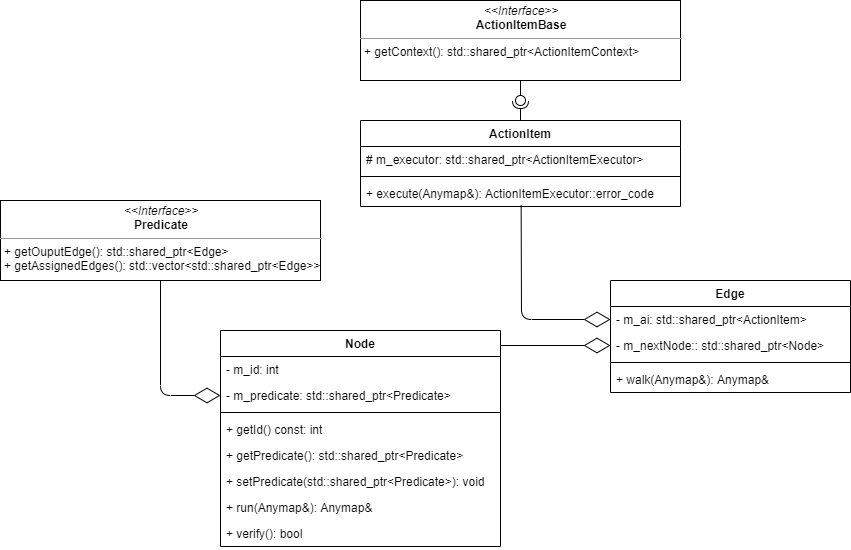
\includegraphics[width=\textwidth]{figures/structure.png}
    \caption{Текущая структура классов, связанная с графовыми моделями в comsdk}
    \label{fig:oldGraphStructure}
\end{figure}

В существующей структуре классов можно выделить следующие недостатки:
\begin{enumerate}[1)]
    \item Отсутствует класс графа, который давал бы удобный интерфейс графовым моделям.
    \item Отсутствует контейнер, который бы инкапсулировал все узлы, относящиеся к конкретной графовой модели.
    \item Индекс узла графа задаётся пользователем при инициализации, что не гарантирует его уникальности.
    \item Отсутствует контейнер, который бы инкапсулировал все рёбра, относящиеся к конкретной графовой модели.
    \item Отсутствует объект, который бы описывал связи между узлами и рёбрами; вместо этого эти связи прописаны в самих узлах и рёбрах, что затрудняет операции с графовой моделью (преобразования и проч.).
    \item Функции-предикаты привязываются к узлам, а не к рёбрам, что не соответствует новым требованиям.
    \item В текущей версии задачей функций-предикатов фактически является отбор рёбер, которые должны быть выполнены, а не проверка соответствия данных в узле определённому формату.
\end{enumerate}

Таким образом, процесс разработки новой структуры графового модуля библиотеки comsdk должен быть направлен как на выполнение требований, описанных в разделе~\ref{section:requirements}, так и на устранение недостатков текущей версии, описанных выше.